%!TEX root = ../../super_main.tex

\chapter{Sprint Conclusion}
\label{cha:conclusion_sprint_4}

The fourth sprint concluded with a presentation to the customers. The two applications we had been working on, along with the other groups' applications, were presented to the customers on a big screen and the customers seemed satisfied with the development. One of the group members during the presentation can be seen in \figref{fig:sprint_review_meeting_presentation}, where he is currently presenting the final state of the \launcher 's home screen.

\begin{figure}[!htbp]
    \centering
    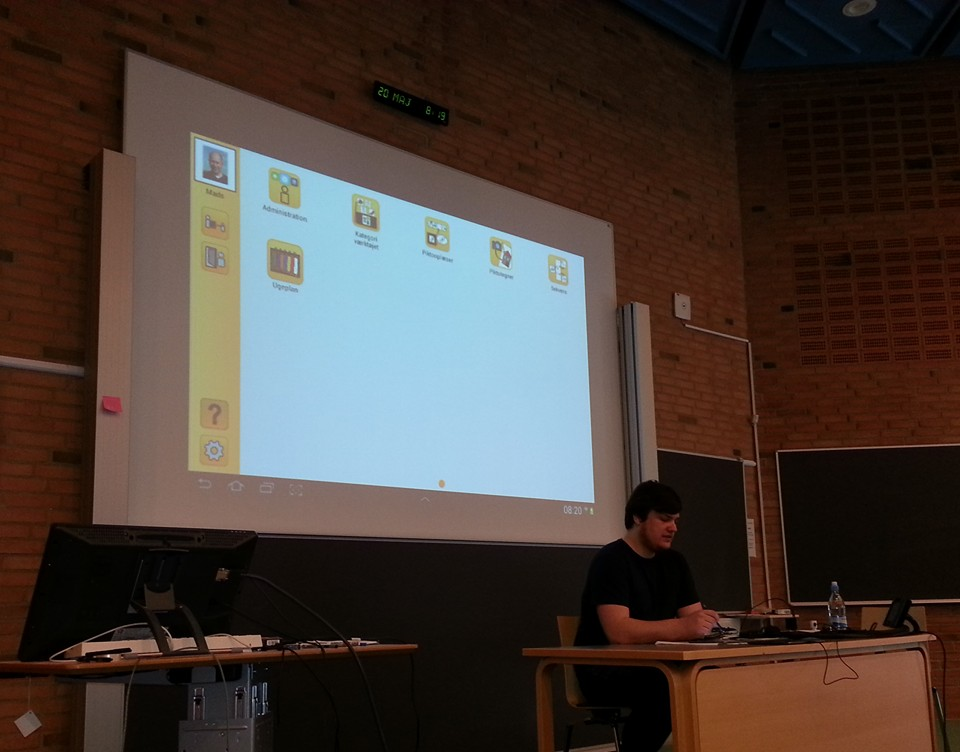
\includegraphics[width=0.75\textwidth]{sprint_four/sprint_review_meeting_presentation}
    \caption{Sprint Review Meeting Presentation}
    \label{fig:sprint_review_meeting_presentation}
\end{figure}

\FloatBarrier

The design manual was completed to a level which describes the design decisions that have been made throughout this semester. This was done in the effort to streamline the \giraf software suite. The design manual includes the design decisions that we found most important, but we have left some open problems, where we had not yet found satisfying solutions, for future \giraf developers to pursue. We encourage future \giraf developers to continue the development of this design manual on the \giraf Git server.
\\\\
In order to assist other groups, we have been actively pursuing them to confront them about not conforming to our design manual and not using the new \gc, as a part of the ``\giraf Police'' responsibility. We also provided support and updated the \gc as more people began to use them and thereby found shortcomings and bugs. 
\\\\
In the early stages of this project we were assigned the responsibility of maintaining the web page \url{www.giraf.cs.aau.dk}. However, during this semester we did not have any user stories from the customers regarding this website and have therefore not been working on it. We did though receive a request from the semester coordinator, \emph{Ulrik Nyman}, that he wanted us to update the favicon of the web page, but we never met this request because we felt that we had more important things to do